\documentclass[a4]{scrartcl}

% \usepackage[ngerman]{babel}
\usepackage[utf8]{inputenc}
\usepackage{mathtools}
\usepackage{amsmath}
\usepackage{amssymb}
\usepackage{geometry}
\usepackage{scrlayer-scrpage}
\usepackage{float}
\usepackage{xcolor}
\pagestyle{scrheadings}
\clearscrheadfoot

\usepackage[backend=biber, maxbibnames=99]{biblatex}
\addbibresource{references.bib}

\setlength{\parindent}{0cm}


\geometry{
  paper=a4paper, % Change to letterpaper for US letter
  top=2cm, % Top margin
  bottom=1.5cm, % Bottom margin
  left=2cm, % Left margin
  right=3cm, % Right margin
}

\ohead{\\
Pina Kolling\\
piko0011}

\usepackage[framemethod=TikZ]{mdframed}

% Style %
\mdfdefinestyle{enviStyle}{
   innertopmargin = 10pt,
  linewidth      = 1pt,
  frametitlerule = true,
  roundcorner    = 2pt%
}


\newenvironment{CountingDefinition}[2][]{%
   \ifstrempty{#1}%
   {\mdfsetup{%
      frametitle={{\strut ~}}}
   }%
   {\mdfsetup{%
      frametitle={{\strut ~#1}}}%
   }%
   \mdfsetup{
      nobreak                   = true,
     linecolor                 = gray,
    frametitlebackgroundcolor = gray!50,
    style                     = enviStyle
   }
   \begin{mdframed}[]\relax%
   \label{#2}}{\end{mdframed}}

\begin{document}

\section*{Summary: Lecture 6}

Summary for the chapter \textit{8.2}. \cite{CC, book}


\subsection*{Completeness}


\begin{CountingDefinition}[]{def:validLabelPlacement}
Let $C$ be a complexity class and let $L$ be a language in $C$. $L$ is called $C$\textit{-complete} if any language $L' \in C$ can be reduced to $L$.
\ \\

(Every language of a complexity class can be reduced to $L$.)
\end{CountingDefinition}



\begin{itemize}
\item reducitbility is transitive $\rightarrow$ problems are ordered by difficulty
\end{itemize}


\color{violet} \textbf{Question: }

Which problems can be reduced to a formal language? 
\begin{itemize}
\item[] \color{black}
\textsc{Sat} can be expressed as formal language. \cite{lang} \\
$\Rightarrow$ \textsc{Sat} can be reduced to a formal language. (?)
\ \\

Because \textsc{Cirquit Sat} can be reduced to \textsc{Sat}: \textsc{Cirquit Sat} can be reduced to a formal language. (?)
\ \\

\begin{CountingDefinition}[Formal language]{def:validLabelPlacement}
Formal languages are abstract languages, which define the syntax of the words that get accepted by that language. It is a set of words that get accepted by the language and has a set of symbols that is called alphabet, which contains all the possible characters of the words. Those characters are called nonterminal symbols. \cite{CNF, language}
\ \\

\textbf{Kleene star} \\
The Kleene star $\Sigma^*$ of an alphabet $\Sigma$ is the set of all words that can be created through concatenation of the symbols of the alphabet $\Sigma$. The empty word $\epsilon$ is included. 
\ \\

\textbf{Formal language}\\
A formal language $L$ over an alphabet $\Sigma$ is a subset of the Kleene star of the alphabet: $L \subseteq \Sigma^*$
\end{CountingDefinition}

Where to set the line between lanuguage decisions and other problems? Can every problem be contrcuted as a formal language?
\ \\

Is everything that is reducable to \textsc{Sat} reducable to a formal language?

\end{itemize}

\color{black}


\begin{itemize}
% \item a reduction definition is usefull because the complexity classe are closed under reduction
\item complete problems can capture the difficulty of a class
\item problem is seen as cpmpletely understood if the problem is complete
\end{itemize}


\begin{CountingDefinition}[Closed under reduction]{def:validLabelPlacement}
The following complexity classes are all closed under reductions:
\begin{itemize}
\item[] \textsc{P} \ \ \  \textsc{NP} \ \ \ \textsc{coNP}
\ \ \ \textsc{L}
\ \ \  \textsc{NL}
\ \ \  \textsc{PSPACE}
\ \ \ \textsc{EXP}
\end{itemize}

A class $C$ is closed under reductions if whenever $L$ is reducible to $L'$ and $L' \in C'$, then $L \ in C'$.
\ \\

If a complete problem in $C$ belongs in a class $C' \subseteq C$, $C = C'$.

\end{CountingDefinition}


\begin{figure}[H]
\begin{center}
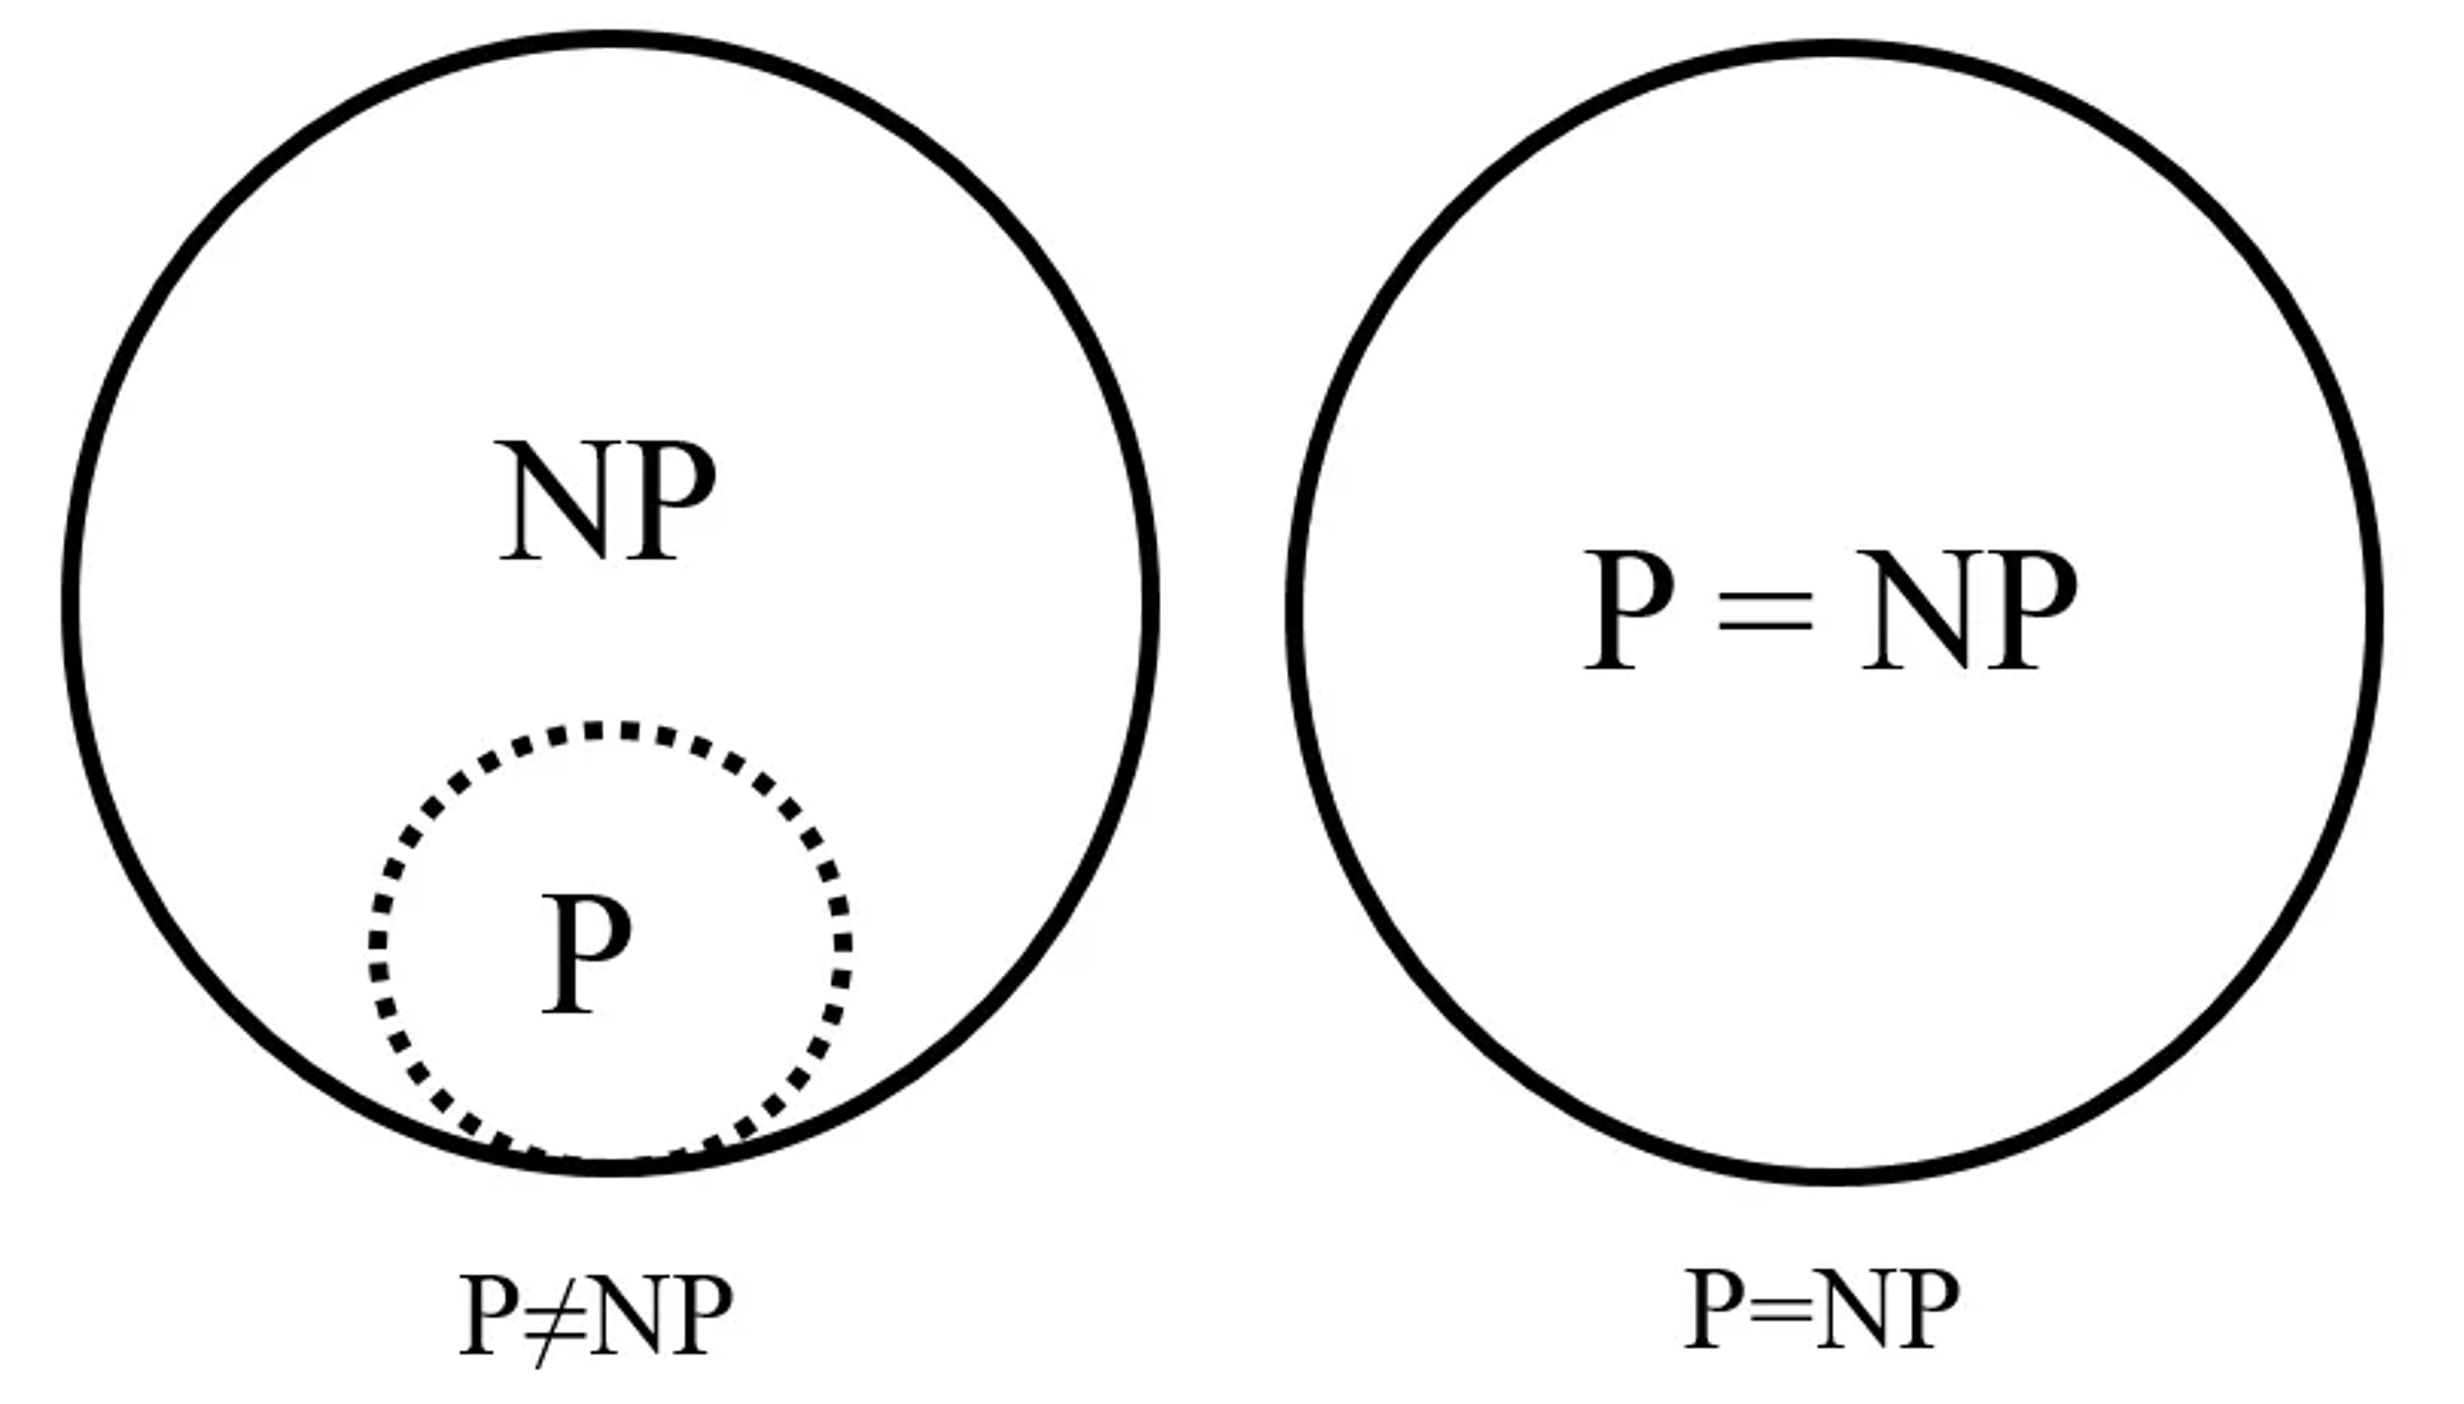
\includegraphics[scale=0.2]{PNP.jpg}
\end{center}
\caption{P and NP sets \cite{PNPsets}}
\end{figure}



\begin{itemize}

\item drawing set circle inclusion thing (\textsc{P} and \textsc{NP})

\end{itemize}


\color{red} TODO \\
\color{black}
\color{violet} Questions:
\color{black}




\subsection*{\textsc{P}-completeness of \textsc{CIRCUIT VALUE}}

\begin{CountingDefinition}[Problem: \textsc{Circuit Value}]{def:validLabelPlacement}
The \textsc{Circuit Value} Problem is the problem of computing the output of a given Boolean circuit on a given input.
\ \\

In terms of time complexity, it can be solved in linear time (topological sort).
\end{CountingDefinition}

\begin{itemize}
\item \textsc{P}-complete
\item limit of power of reductions
\item got a little tired and zoned out
\end{itemize}



\color{red} TODO \\
\color{black}
\color{violet} Questions:
\color{black}





\subsection*{The reduction (?)}

\begin{CountingDefinition}[Problem: \textsc{Circuit Sat}]{def:validLabelPlacement}
The circuit satisfiability problem (\textsc{Circuit Sat}) is the decision problem of determining whether a given Boolean circuit has an assignment of its inputs that makes the output true.
\ \\

Input: a Boolean circuit $C$ 
\ \\

Question: Is there a truth assignment which makes $C$ output the value true?
\end{CountingDefinition}





\subsection*{\textsc{CIRCUIT SAT} is \textsc{NP}-complete}

\begin{itemize}
\item circuit decides nondeterministically (?)
\item a variable is added n the nondeterministic Turing Machine
\item check if one of the variables is tue: use this choice (?)
\item problem: can we set thiese variables such that the Turing Machine accepts?
\item answer corresponds direct to \textit{is there a choice of nd decisions such that the turing machine accepts?}
\item extremely direct reduction
\item cooks theorem :) 
\item \textsc{SAT} is \textsc{NP}-complete
\end{itemize}




\color{red} TODO \\
\color{violet} Questions:
\color{black}


\newpage

\printbibliography




\end{document}